\section{Results} \label{sec:results}

% overview of runs
An overview of the experimental runs is given in Fig. \ref{fig:run123}. The figure shows a set of six views of information for each run. These views are created at every iteration and generate a movie of the run. Fig. \ref{fig:run123} shows a snapshot of these views at different points of the simulation for each run. The views are described below:

\begin{itemize}
  \item Top Left - View of the global mesh $M$ from a third perspective. The
  wire frame corresponds to the viewing frustum of the sensor. The light blue
  helical line is the path of the sensor. Gray is the simulated environment.
  The multi-colored mesh is the global mesh $M$. The mesh is multi-colored in order
  to show the passage of time. For example, in Run1, The mesh is colored yellow,
  light green, and dark green for iterations 1, 2, and 3 respectively.
  \item Top Middle - Same as Top Left except it shows the novel surface $S$ instead of
  the global mesh $M$.
  \item Top Right - Plot showing the number of elements in the global mesh $M$
  up to this iteration.
  \item Bottom Left and Bottom Middle - Actual $D$ and expected $E$ depth image
  respectively.
  \item Bottom Right - The classified depth image. Novel point $D_n$ are shown
  in black. Points to be thrown away are shown in white.
\end{itemize}

We can notice important aspects of MABDI using Fig. \ref{fig:run123}. Notes on each of the runs:

\begin{itemize}
  \item Run 1 - Top Left shows how the $M$ gets composed over time.
  It is important to note that the mesh is not overlapping itself. This can be
  understood by noticing $S$ from Top Middle is the same as
  the section of $M$ this is colored dark green.
  \item Run 2 - This run shows clearly how the classification process is able to
  distinguish novel points. This can be seen by noticing the valley in-between
  the ear and the eye of the bunny closest to the sensor. The sensor was not
  able to see these points from the prior iteration due to occlusion. From the
  sensor's current perspective, the points can now be seen. Notice how the
  valley is missing in the \emph{expected} depth image $E$, classified as novel
  in Bottom Right, and thus reconstructed into $S$. This is a clear example of
  the concept behind MABDI.
  \item Run 3 - This run shows how MABDI reacts to object addition. At this
  iteration the middle bunny is suddenly added. We can follow the data: $D$
  shows the new bunny, $E$ shows what we expect to see (the middle bunny is not
  there because it is not in $M$), Bottom Right shows all points corresponding
  to the new bunny as marked as novel, and finally the novel points are
  reconstructed as $S$ and appended to $M$. Top Right also shows a large jump in
  the number of elements in $M$ due to the new bunny.
\end{itemize}

% global mesh
Fig \ref{fig:gm} shows the resultant global mesh from all of the runs along with a plot of the number of elements in the mesh over iterations. These plots show the main contribution of MABDI because they level-off as the environment becomes more known as opposed to traditional ``black box'' reconstruction methods where the number of elements increases linearly over time.

\begin{figure}[h]%[thpb]
\centering
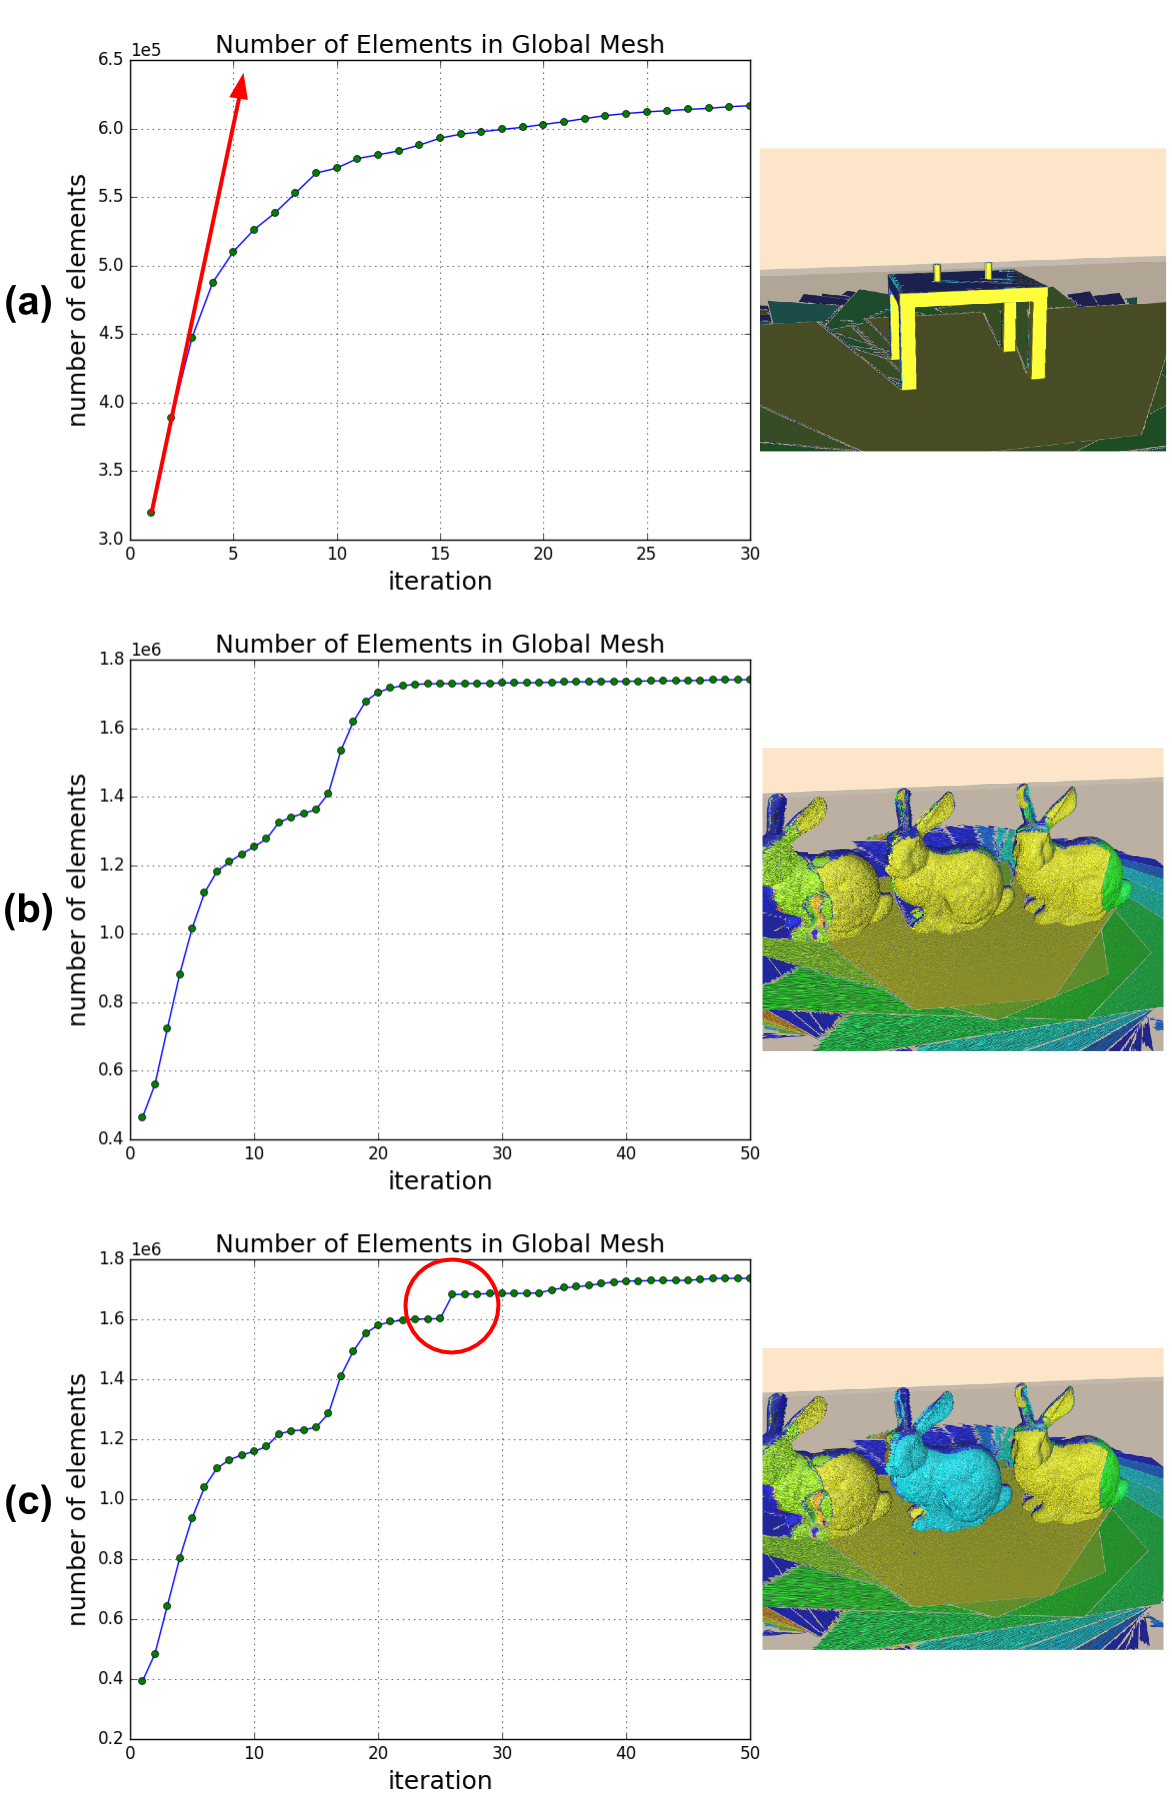
\includegraphics[width=0.48\textwidth]{figures/diagram_run123_gm.png}
\caption{Global mesh results. Top: Run1. Middle: Run2. Bottom: Run3}
\label{fig:gm}
\end{figure}
